\chapter{Diseño de la interfaz de explicaciones}
\label{cap:interfaz}

A la hora de pensar en el tipo de interfaz gráfica tenemos que tener en cuenta el método de almacenamiento de datos, su formato y por último cual es la mejor manera de representarlos gráficamente. En nuestro caso los datos se basan en objetos y sus relaciones que tienen entre sí por lo que creemos que la mejor representación que podemos elegir es mediante un grafo.
En este grafo queremos plasmar todos los caminos que han sido seleccionados navegando por el formato RDF que proporciona la web Wikidata. De esta forma solo incluiremos en el diseño aquellos caminos que lleven a una propiedad que compartan ambas canciones, con la intención de representar cada uno de ellos.

\begin{figure}[h!]
	\centering
	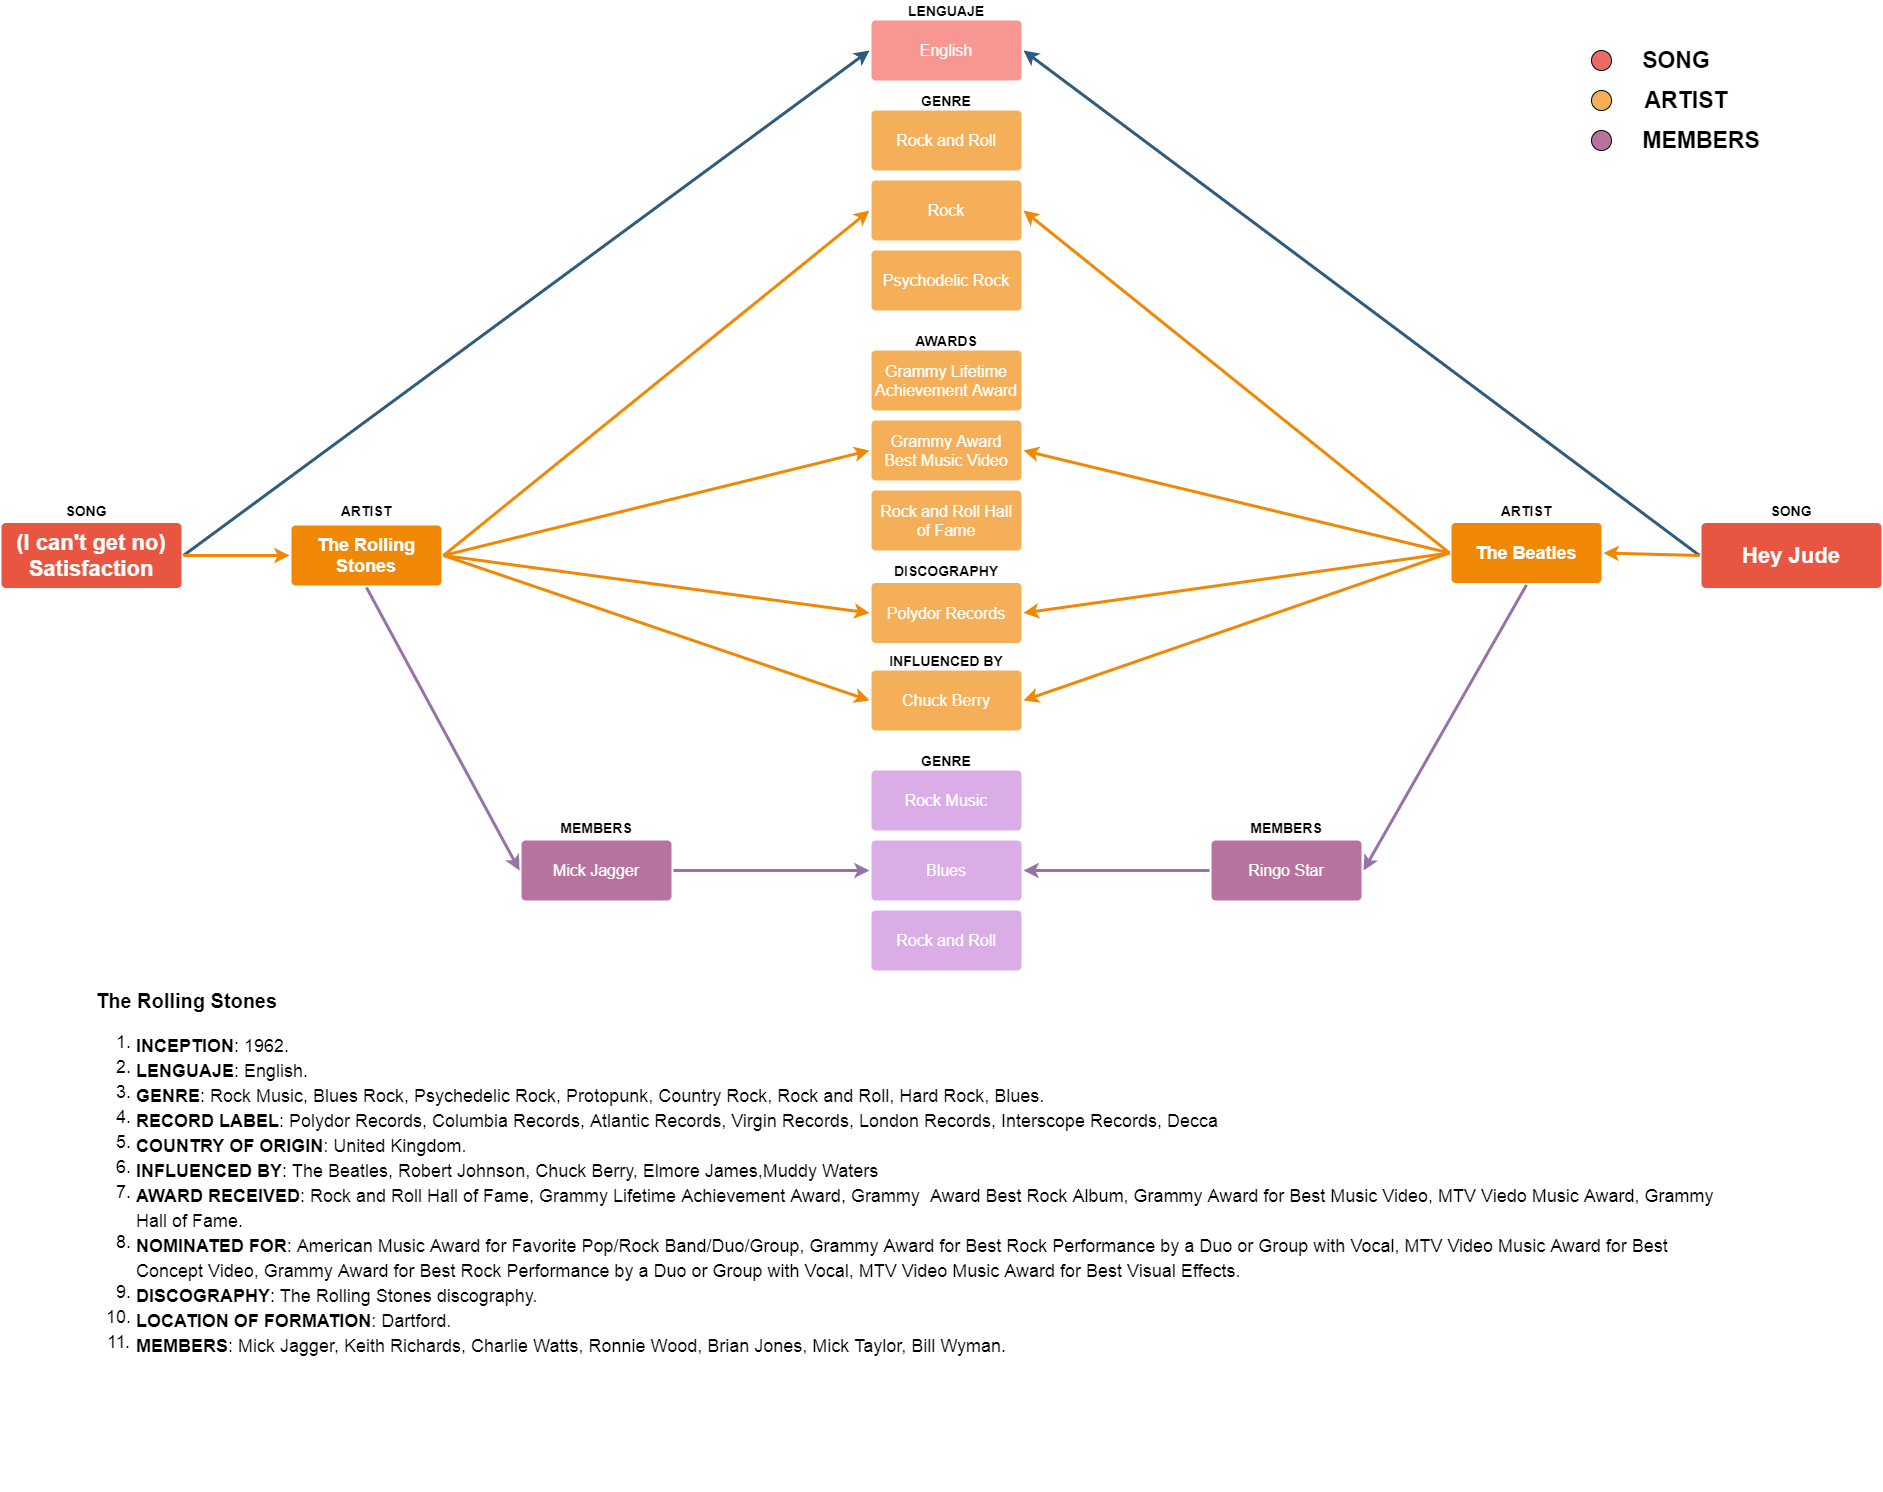
\includegraphics[width = 1\textwidth]{Imagenes/Bitmap/InterfaceResult.png}
	\caption{Primer diseño de la interfaz web}
	\label{fig:sampleImage}
\end{figure}

Para poder explicar la interfaz, se debe explicar las dos ramas principales que ejecutamos a la hora de realizar el estudio. El objeto de cada una de estas ramas es el título de las dos canciones que queremos estudiar. Cada rama o camino empieza estudiando las propiedades de cada una de las canciones, a partir de ahí, se navegará por cada una de las siguientes propiedades hasta que ambas ramas se junten en una misma propiedad común.
Lo ideal sería poder representar claramente los tres primeros niveles que hasta el momento hemos considerado y hacer la representación de cada uno de ellos.

Tomando en cuenta las explicaciones dadas sobre los niveles o complejidad que hemos recogido, suponiendo que hay relaciones compartidas en todos ellos obtendríamos los siguientes grafos:
- Tenemos tres niveles en cada canción.
- Suponemos que cada nivel de la canción 1 puede relacionarse con todos los niveles de la canción 2. Así pues la propiedad género de la canción 1 (nivel 1) puede estar ligada a la propiedad género del artista(nivel 2) de la canción 2 o a la propiedad género un miembro de la banda que toca la canción 2 (nivel 3).
- Se pueden representar un máximo de 9 grafos (3\^2).

Como información extra y con un carácter meramente informativo, consideramos una extensión que pueda mostrar toda la información recogida sobre cada objeto que aparece en el grafo. Asi al hacer click sobre un objeto, ya sea un artista, un género o una canción, se muestre una extension que muestre todas las relaciones que hemos recopilado sobre ese objeto, incluidas las no compartidas por la otra rama de la segunda canción.